\chapter{Proposed Algorithm and Architecture}
\label{paaa}
\section{Profiling an LSTM}
Since the primary objective of our work is to develop an implementation of an LSTM on hardware with minimal power, compute and memory requirement, we will need to first identify what operations in the network's structure occupies the most compute power. The following methodology was adopted to profile the LSTM.\\
A 2 Layer LSTM with 128 hidden units each was implemented in $Tensorflow$, a computation graph library for deep neural networks and the $Profiler$ tool of the library was used to find the number of floating-point operations(FLOPs) each broad category of operation required. The results are represented graphically below.

\begin{figure}[h]
\caption{Profile of LSTM Network}
\centering
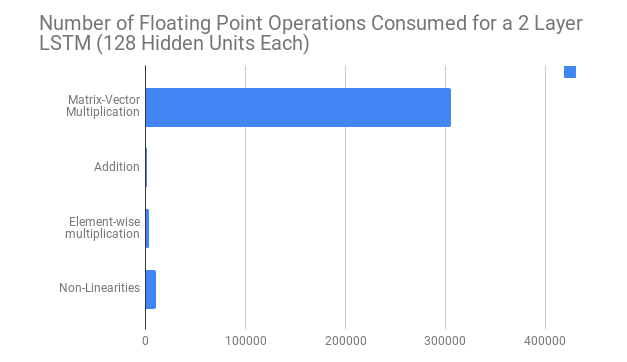
\includegraphics[width=0.8\textwidth]{profile}
\end{figure}

The following conclusions can be drawn from the above graph:
\begin{itemize}
    \item The most computationally expensive operation is the \textbf{matrix-vector multiplication}. Of the matrix and the vector, the vector or the input changes every time instant but the matrix is constant for a particular network regardless of the input. This needs to leveraged when optimizing the network
    \item The next most computationally expensive operation are the \textbf{non-linearities} $sigmoid$ and $tanh$.
    \item \textbf{Element-wise multiplication} and \textbf{addition} operations are insignificant in comparison with the other operations.
\end{itemize}

\section{Matrix-Vector Multiplication}
constant matrix and matmul is the most expensive operation. leads to DA being a possible option

As mentioned above, the matrix-vector multiplication operation is the one that needs to be tackled first. Since the weight matrices are constant for a particular network, distributed arithmetic can be seen as a possible solution to implement the multiplication operation. DA removes the need for a multiplier in the circuit. Therefore, below, DA and its various optimizations are elaborated and applied to task of matrix-vector multiplication. The memory requirement is then analysed and further avenues to reduce this are proposed.
\subsection{Distributed Arithmetic}
\subsubsection{Offset Binary Coding}
\subsubsection{ROM Decomposition}
\subsubsection{Applying DA to LSTMs}
tell the current memory requirement
\subsection{Network Compression}
\subsubsection{Pruning}
\subsubsection{Quantization}
\subsubsection{Low Displacement Rank Methods}
\subsubsection{Knowledge Distillation}
\subsubsection{Logic Based without DA}

-Pruning creates 90\% sparsity. Is it possible to exploit??? cite the sparse DA paper.
-Quantization - need to store less, but indexing is more problematic
-Knowledge Distillation has shown to reduce model size ~5x( read the paper)
-No memory, direct logic gates
